\documentclass[tikz,border=2pt]{standalone}
\usepackage{amsmath}
\usepackage{pgfplots}
\pgfplotsset{compat=1.18}

\begin{document}
% Partial sums of 1 - 1/2 + 1/3 - 1/4 + ... swing from one side of the limit to the other,
% each swing smaller than the last.
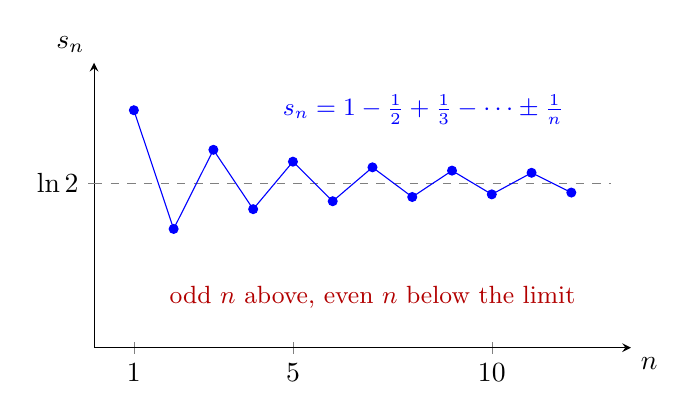
\begin{tikzpicture}
	\begin{axis}[
		axis lines=middle,
		xmin=0, xmax=13.5,
		ymin=0, ymax=1.2,
		xtick={1,5,10}, ytick={0.693}, yticklabels={$\ln 2$},
		xlabel={$n$}, ylabel={$s_n$},
		xlabel style={below right}, ylabel style={above left},
		clip=false,
		width=8.4cm, height=5.2cm
		]
		\addplot[gray, dashed, domain=0:13] {0.6931};
		\addplot[blue, thin, mark=*, mark size=1.6pt] coordinates {
			(1,1) (2,0.5) (3,0.8333) (4,0.5833) (5,0.7833) (6,0.6167) (7,0.7595) (8,0.6345) (9,0.7456) (10,0.6456) (11,0.7365) (12,0.6532)
		};
		\node[blue, anchor=south west, font=\small] at (axis cs:4.5,0.9) {$s_n=1-\tfrac12+\tfrac13-\cdots\pm\tfrac1n$};
		\node[red!70!black, anchor=north, font=\small] at (axis cs:7,0.3) {odd $n$ above, even $n$ below the limit};
	\end{axis}
\end{tikzpicture}
\end{document}
